%% about_me.tex
%% Author: Leighton Pritchard
%% Copyright: James Hutton Institute
%% Why should anyone listen to me, regarding visualisation

% POTTED CV
\begin{frame}
  \frametitle{What I do}
      \begin{itemize}  
        \item \textcolor{hutton_green}{Computational biologist (1996-present)}
        \begin{itemize}
          \item protein sequence-structure-function (1996-1999)
          \item yeast metabolism (1999-2003)
          \item plant pathology (2003-present)
        \end{itemize}
        \item \textcolor{hutton_blue}{Large datasets}
        \begin{itemize}
          \item sequence/genomic
          \item metabolomics
          \item statistics
          \item geographical
        \end{itemize}
        \item \textcolor{hutton_purple}{Visualisation as communication to (wet) biologists}
        \begin{itemize}
          \item protein structures
          \item metabolic flux
          \item comparative genomics/evolution
          \item statistical plots
        \end{itemize}
      \end{itemize}  
\end{frame}

% GENOMEDIAGRAM
\begin{frame}
  \frametitle{GenomeDiagram 
    \footnote{\tiny{\href{http://dx.doi.org/10.1093/bioinformatics/btk021}{Pritchard \textit{et al.} (2006) \textit{Bioinformatics} doi:10.1093/bioinformatics/btk021}}}
    \footnote{\tiny{Toth \textit{et al}. (2006) \textit{Ann. Rev. Phytopath.} \href{http://dx.doi.org/10.1146/annurev.phyto.44.070505.143444}{doi:10.1146/annurev.phyto.44.070505.143444}}}
    \footnote{\tiny{\href{http://biopython.org}{http://biopython.org}}}
    
\includegraphics[width=0.18\textwidth]{images/biopython}
  }
  \begin{center}
      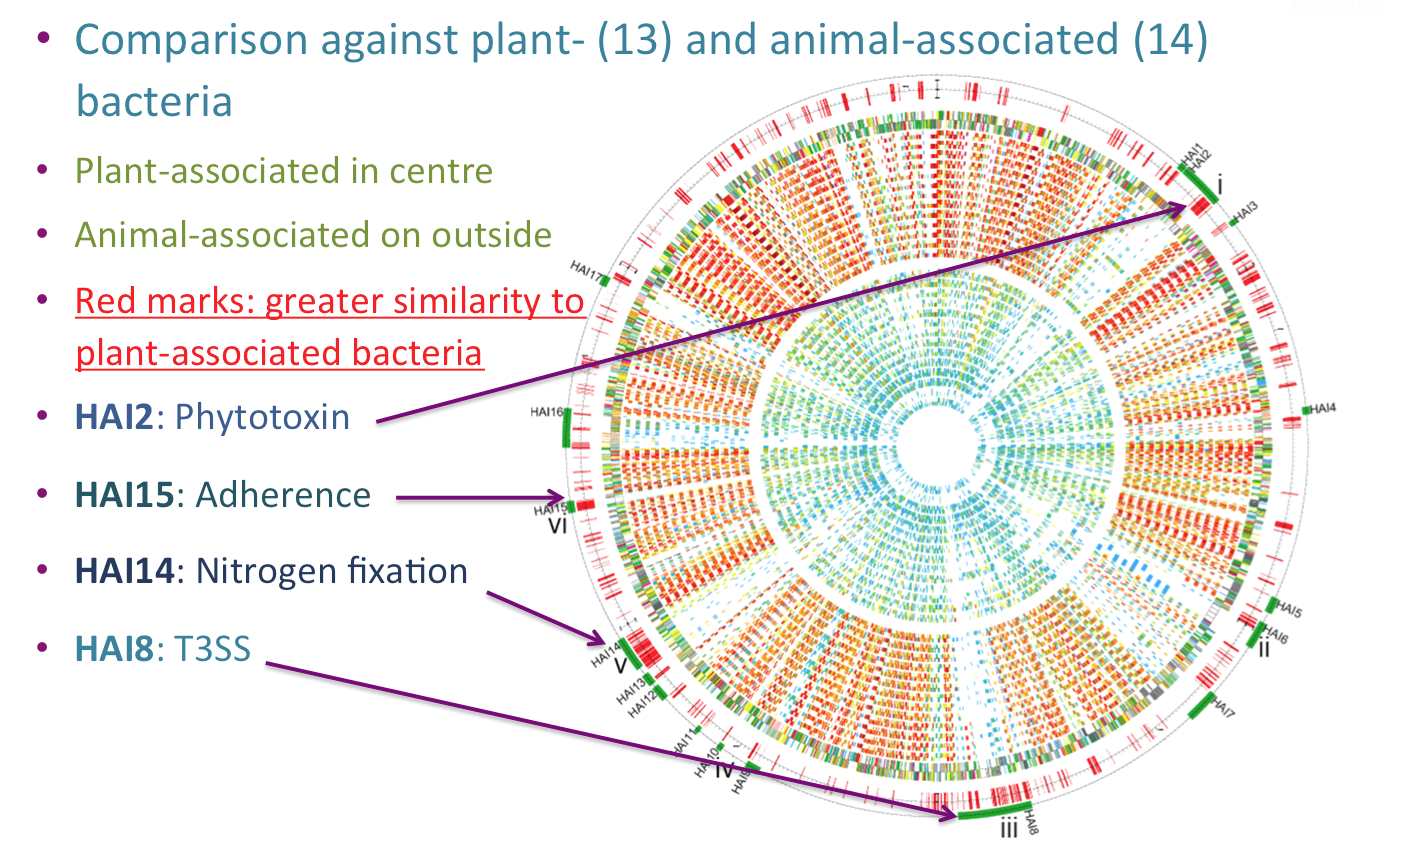
\includegraphics[width=0.9\textwidth]{images/pba_lgt} 
  \end{center}
\end{frame}

% CORONATINE
\begin{frame}
  \frametitle{Functional adaptation in \textit{Pba}
    \footnote{\tiny{Toth \textit{et al}. (2006) \textit{Ann. Rev. Phytopath.} \href{http://dx.doi.org/10.1146/annurev.phyto.44.070505.143444}{doi:10.1146/annurev.phyto.44.070505.143444}}}
    \footnote{\tiny{\href{http://biopython.org}{http://biopython.org}}}
  }
  \begin{center}
      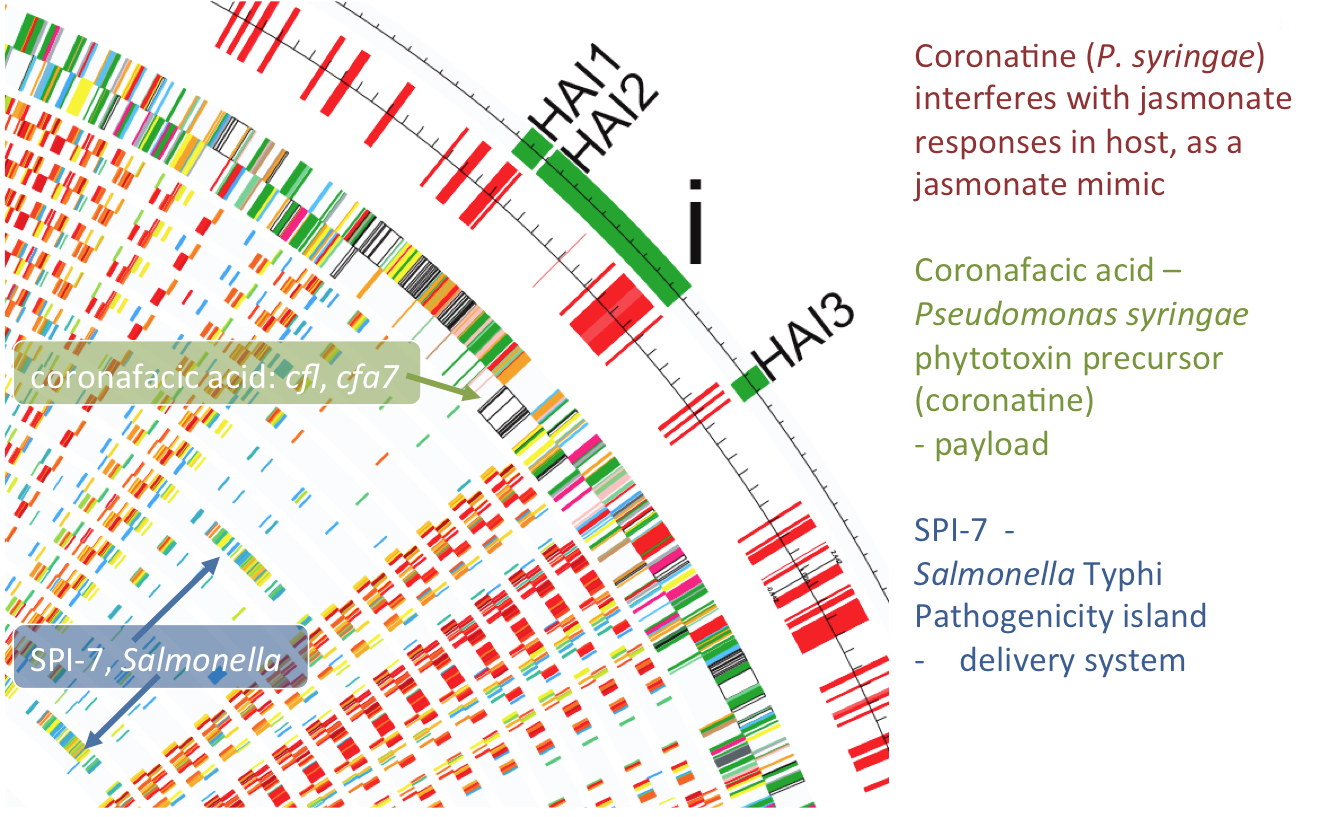
\includegraphics[width=1\textwidth]{images/pba_coronatine} 
  \end{center}
\end{frame}

%% GENOMEDIAGRAM/BIOPYTHON
\begin{frame}
  \frametitle{GenomeDiagram/SciArt
  \footnote{\tiny{\href{http://dx.doi.org/10.1093/bioinformatics/btk021}{Pritchard \textit{et al.} (2006) \textit{Bioinformatics} doi:10.1093/bioinformatics/btk021}}}
  \footnote{\tiny{Shemilt (2009) in``Digital Visual Culture: Theory and Practice'' ISBN 978-1-84150-248-9}}
  \footnote{\tiny{Shemilt (2010) in ``Art Practice in a Digital Culture'', ISBN 978-0-7546-7623-2}}
  }
  \begin{columns}[T]
    \begin{column}{3.5cm}  
%      \includegraphics[height=0.3\textheight]{images/gd_large} \\
      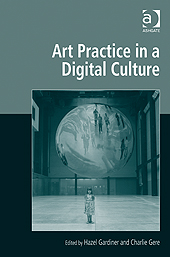
\includegraphics[height=0.4\textheight,center]{images/art_practice}      
        \begin{tiny}    
          \begin{alertblock}{Influence}
            Free open-source comparative genomics visualisation library
          \end{alertblock}                
        \end{tiny}          
        
\includegraphics[width=1\textwidth]{images/biopython}          
    \end{column}    
    \begin{column}{3.5cm}  
      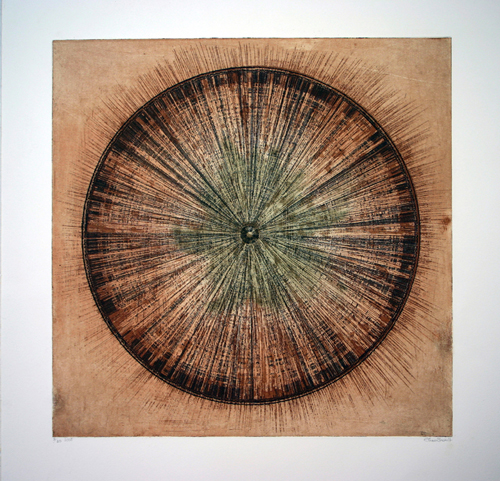
\includegraphics[height=0.4\textheight]{images/shemilt-fig3} \\
        \begin{tiny}        
          \begin{alertblock}{Impact}
            Artwork (prints, audio-visual installation) exhibited in UK and internationally
          \end{alertblock}                
        \end{tiny}                        
    \end{column}
    \begin{column}{3.5cm}  
      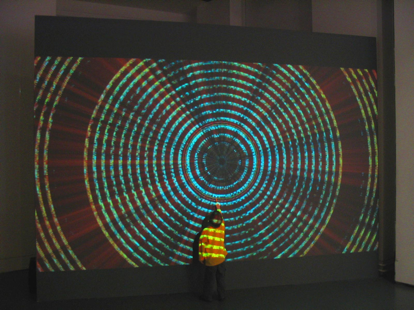
\includegraphics[width=1\textwidth]{images/sciart2} \\
      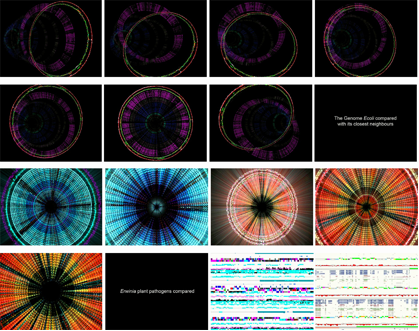
\includegraphics[width=1\textwidth]{images/sciart3}
    \end{column}  
  \end{columns}
\end{frame}

% KGML/KEGG 
\begin{frame}
  \frametitle{Comparative metabolism
    \footnote{\tiny{\href{https://github.com/widdowquinn/notebooks/blob/master/Biopython_KGML_intro.ipynb}{Biopython KGML/KEGG visualisation module}}}
    \footnote{\tiny{\href{https://github.com/widdowquinn/Notebooks-Bioinformatics}{https://github.com/widdowquinn/Notebooks-Bioinformatics}}}
    \footnote{\tiny{\href{http://biopython.org}{http://biopython.org}}}    
    
\includegraphics[width=0.18\textwidth]{images/biopython}
  }
  \begin{center}
    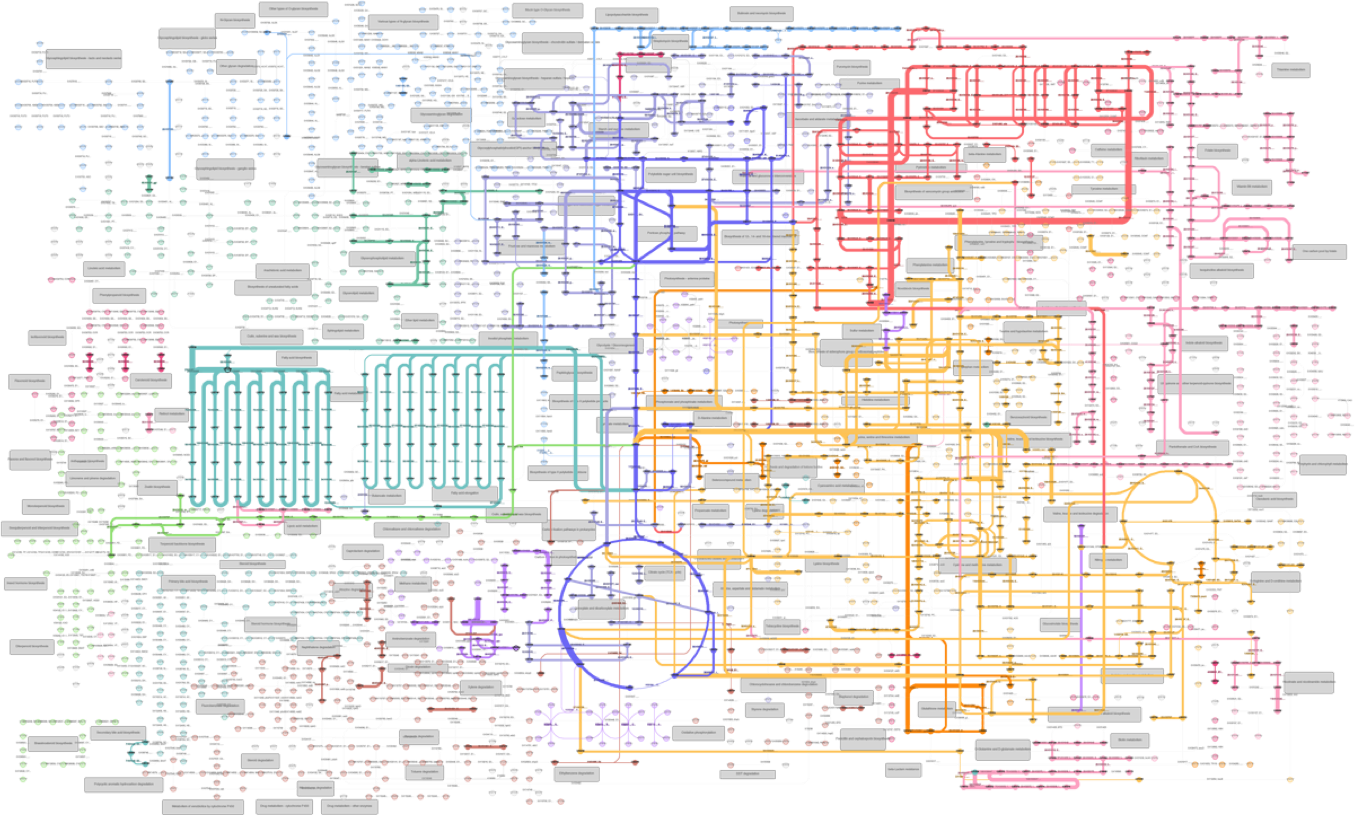
\includegraphics[width=0.9\textwidth]{images/dickeya_pathways}
  \end{center}
\end{frame}

% PYANI
\begin{frame}
  \frametitle{PyANI: prokaryote classification
  \footnote{\tiny{\href{http://widdowquinn.github.io/pyani/}{http://widdowquinn.github.io/pyani/}}}
  \footnote{\tiny{\href{http://dx.doi.org/10.1039/C5AY02550H
}{Pritchard \textit{et al.} (2016) \textit{Anal. Methods} doi:10.1039/C5AY02550H
}}}  
  }
  \begin{center}
    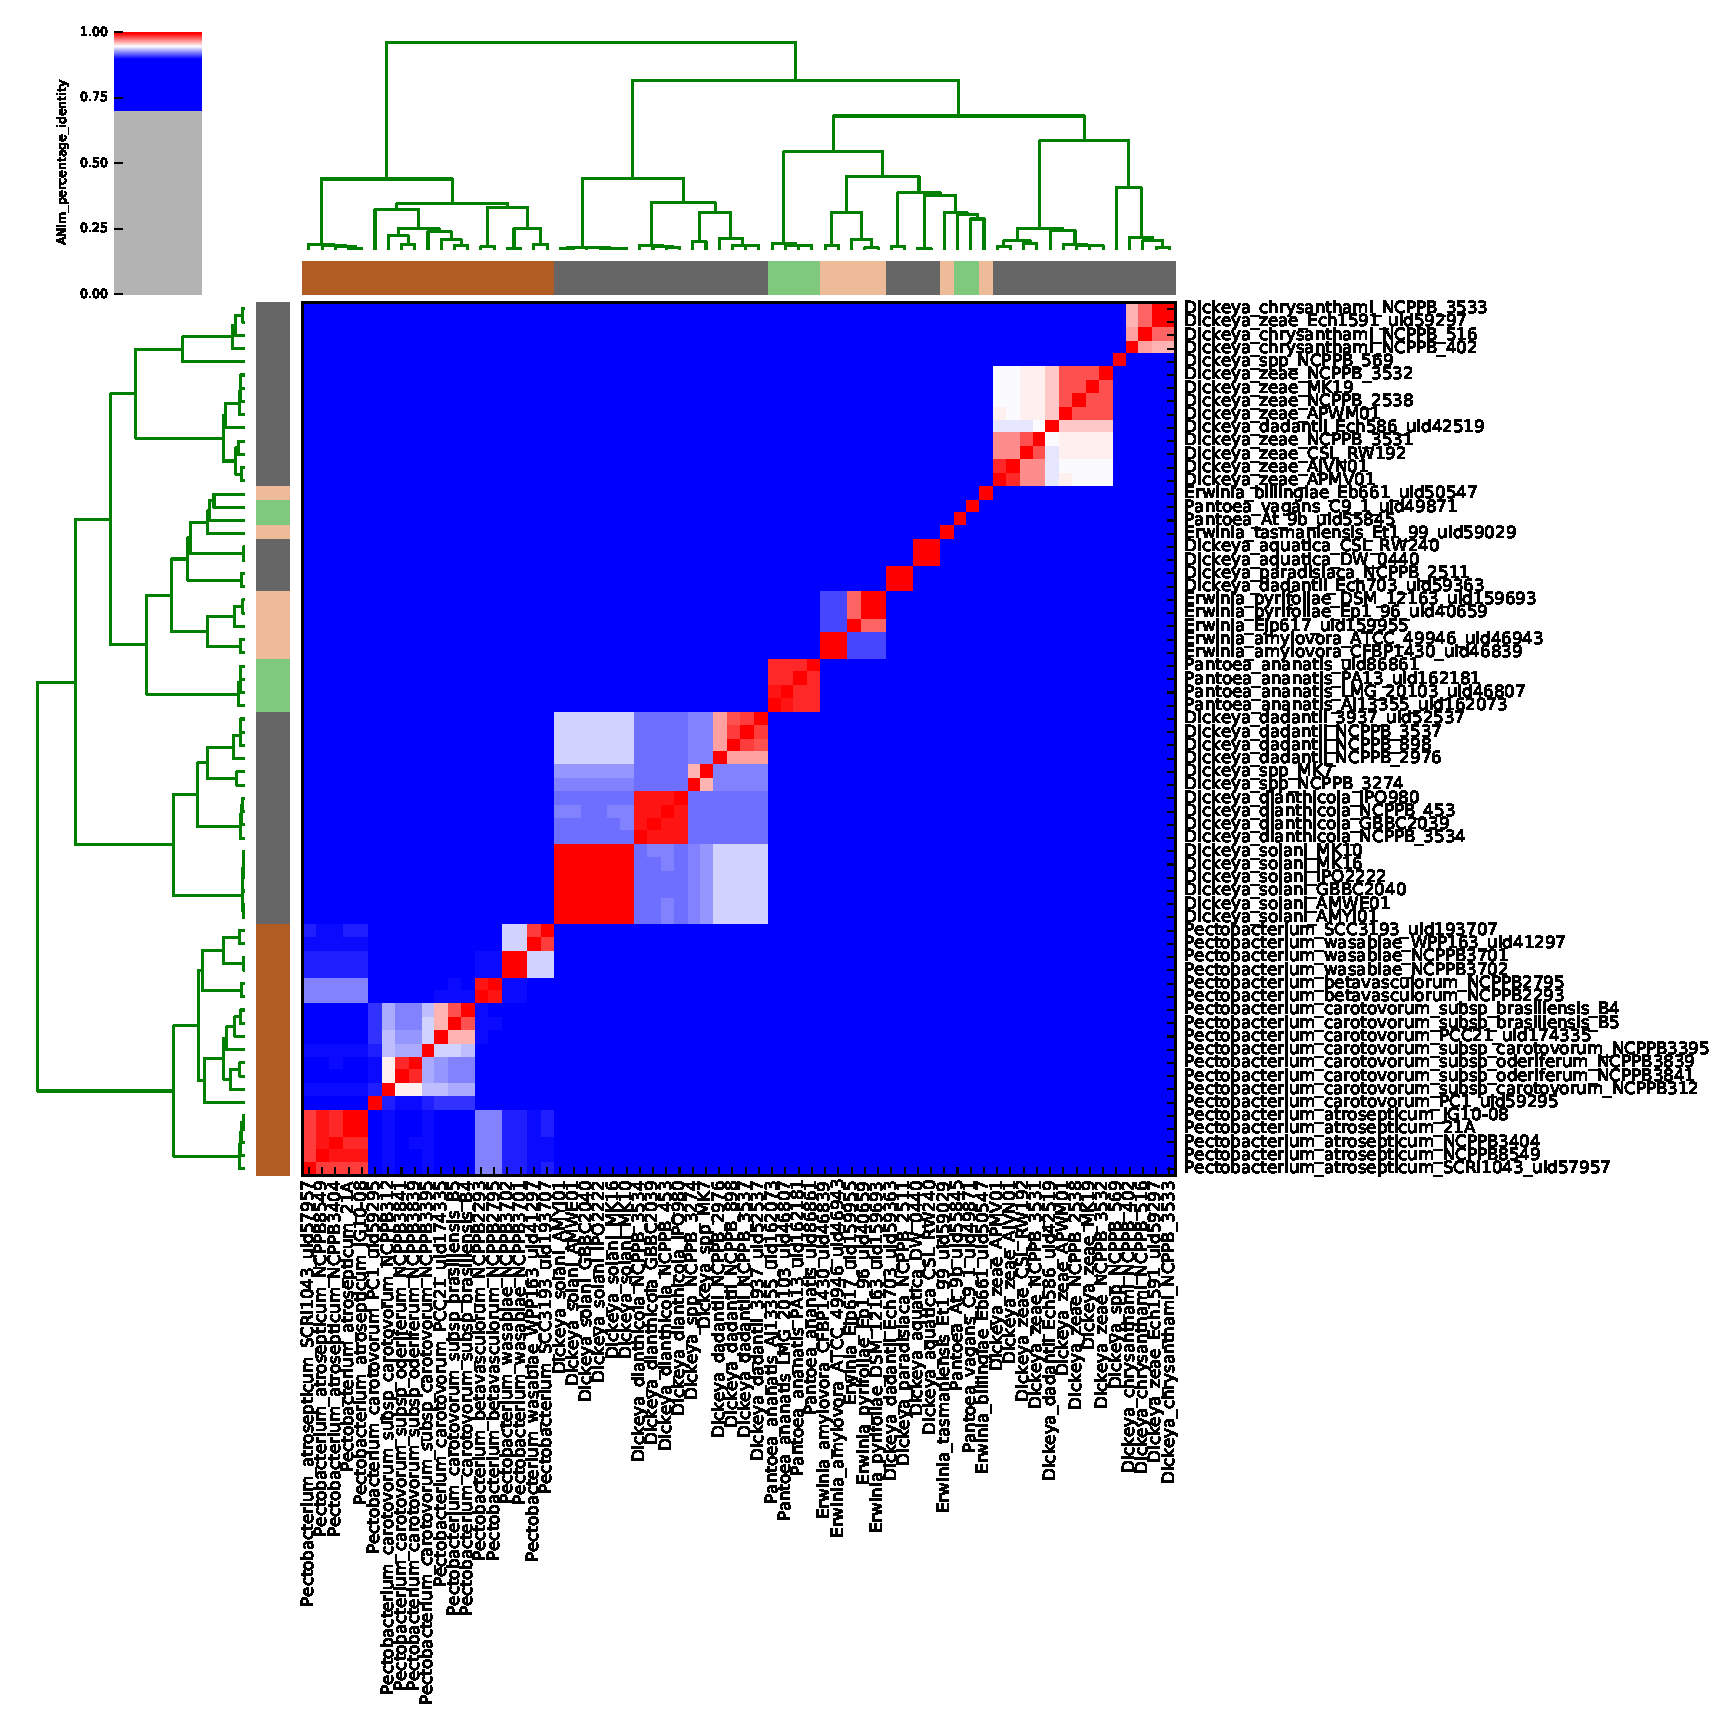
\includegraphics[height=0.75\textheight]{images/figure_anim_pid_SRE}
  \end{center}
\end{frame}